\chapter{Image processing}

\noindent
La forma más sencilla de entender una imagen digital es como una matriz de valores de intensidad. Cada celda de la matriz se llama píxel (picture element). En una imagen de escala de grises estándar de 8 bits, estos valores oscilan entre 0 (negro total) y 255 (blanco total). Lo que nosotros percibimos como formas y texturas, el ordenador lo interpreta como una tabla de números donde los valores altos representan zonas claras y los bajos zonas oscuras. \\ \\
\noindent
Para poder aplicar herramientas matemáticas (como las derivadas que usaremos para detectar bordes), definimos la imagen como una función bidimensional:
$$f(x, y)$$
donde 
\begin{itemize}
    \item $(x, y)$ son las coordenadas espaciales (la posición del píxel en la columna $x$ y fila $y$).
    \item $f$: Es la amplitud o intensidad en ese punto.
\end{itemize}
Si estuviéramos trabajando con una imagen continua (analógica), $f$ sería una función definida sobre un plano real. Sin embargo, en el mundo digital, trabajamos con una función discreta, donde $x$ e $y$ son números enteros (índices de la matriz).


\section{Point Processing}
\noindent 
Entender concepto solo, no es necesario memorizar fórmulas (no es pregunta de examen). 

\subsection{Gamma Correction}
\noindent
La \tbf{Gamma Correction} es una operación de punto (point operation) no lineal que ajusta la relación entre el valor del píxel y la intensidad real de luz. La fórmula fundamental que rige este proceso es la ley de potencia
$$V_{out} = A \cdot V_{in}^{\gamma}$$
donde
\begin{itemize}
    \item $V_{in}$: Es el valor de intensidad de entrada (normalizado entre 0 y 1).
    \item $V_{out}$: Es el valor de intensidad de salida.
    \item $\gamma$ (Gamma): Es el exponente que define la forma de la curva de transformación.
    \item $A$: Es una constante (normalmente 1 en cálculos normalizados).
\end{itemize}

\subsection{Histogram Equalization}
\noindent
A veces, una imagen tiene todos sus píxeles concentrados en un rango muy estrecho de valores (por ejemplo, una imagen muy oscura donde todos los píxeles están entre 0 y 50), por lo que tiene poca variación de intensidad, es decir, poco contraste. El \tbf{histograma} de esta imagen mostraría una gran ``montaña'' en la izquierda y nada en el resto. \\

\noindent
La \tbf{ecualización del histograma} busca una función de transformación $T$ tal que el histograma de la imagen de salida sea lo más plano (uniforme) posible. Esto significa que queremos que cada nivel de gris tenga, idealmente, el mismo número de píxeles. Esto maximiza el contraste. \\
\noindent
Para lograr esto, utilizamos una herramienta estadística llamada \tbf{Función de Distribución Acumulada} (en inglés, CDF - Cumulative Distribution Function). La receta matemática es la siguiente:

\begin{enumerate}
    \item \underline{Calcular el histograma} de la imagen original $p(r_k)$, que nos dice cuántos píxeles hay de cada valor $r_k$
    \begin{equation*}
        p(r_k) = \frac{\text{Number of pixels with intensity } r_k}{\text{Total number of pixels } n}
    \end{equation*}
    \item \underline{Normalizar el histograma}, que viene a ser calcular la función CDF del histograma
    \begin{equation*}
        CDF(r_k) = \sum_{j=0}^{k} p(r_j)
    \end{equation*}
    \item \underline{Aplicar la transformación} a cada píxel de la imagen original para obtener la imagen ecualizada. La CFD se normaliza de tal manera que los valores mínimo y máximo del CDF corresponden a los valores mínimos y máximos posibles de intensidad (0 y 255 para una imagen de 8 bits)
    \begin{equation*}
        r_k'=round\left(\dfrac{(CDF(r_k)-CDF_{min})\cdot (L-1)}{N-CDF_{min}}\right)
    \end{equation*}
    donde
    \begin{itemize}
        \item $r_k'$: Es el nuevo valor de intensidad para el píxel con valor original $r_k$.
        \item $CDF_{min}$: Es el valor mínimo de la CDF (correspondiente al primer nivel de gris que tiene píxeles).
        \item $L$: Es el número total de niveles de gris (por ejemplo, 256 para imágenes de 8 bits).
        \item $N$: Es el número total de píxeles en la imagen.
    \end{itemize}
\end{enumerate}
En la Figura \ref{fig:histogram_equalization} se muestra un ejemplo de cómo la ecualización del histograma mejora el contraste de una imagen al distribuir los valores de intensidad de manera más uniforme a lo largo del rango disponible. La imagen original tiene un histograma concentrado en un rango estrecho, mientras que la imagen ecualizada tiene un histograma más uniforme, lo que mejora el contraste visual.

\begin{figure}[h]
    \centering
    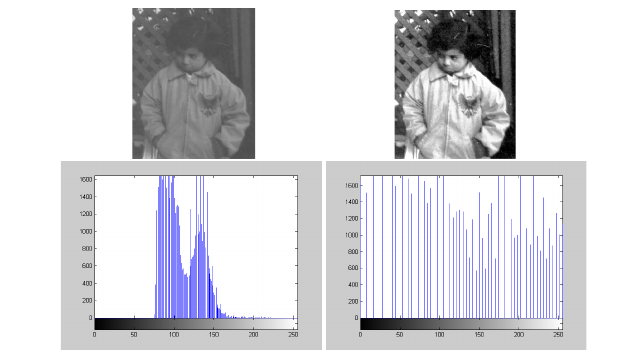
\includegraphics[width=0.8\textwidth]{img/histogram_equalization.png}
    \caption{Ejemplo de ecualización de histograma. La imagen original tiene un histograma concentrado en un rango estrecho, mientras que la imagen ecualizada tiene un histograma más uniforme, lo que mejora el contraste.}
    \label{fig:histogram_equalization}
\end{figure}


\section{Linear filtering}

\noindent
El filtrado lineal es una técnica donde cada píxel de una imagen es reemplazado por una combinación lineal (una suma ponderada) de sus píxeles vecinos. La ``receta'' que define los pesos de esta combinación se conoce como \tbf{kernel, máscara o filtro}. \\

\noindent
Existen dos operaciones matemáticas fundamentales para aplicar estos filtros: la \tbf{correlación cruzada} y la \tbf{convolución}.

\subsection{Correlación Cruzada (Cross-correlation)}
\noindent
Matemáticamente, puede entenderse como un ``producto punto'' entre el vecindario local de la imagen y el kernel. Si $F$ es la imagen original, $H$ es el kernel (de tamaño $(2k+1) \times (2k+1)$) y $G$ es la imagen resultante, la operación se define como:
\begin{equation*}
    G[i,j]= \sum_{u=-k}^{k} \sum_{v=-k}^{k} H[u,v]F[i+u,j+v]
\end{equation*}
\noindent
Propiedad matemática: Esta operación no es asociativa ni conmutativa, lo que significa que el orden de aplicación de los filtros importa, y no se pueden reordenar sin cambiar el resultado. Esto es importante a tener en cuenta al diseñar cadenas de procesamiento de imágenes, ya que aplicar los filtros en un orden diferente puede producir resultados significativamente distintos.

\subsection{Convolución (Convolution)}

\noindent
Es la operación estándar en el procesamiento de imágenes. Es idéntica a la correlación cruzada, con una única diferencia crítica: el kernel $H$ se invierte (se voltea horizontal y verticalmente) antes de realizar la suma ponderada. Se denota con el símbolo $\ast$ y su fórmula es:
\begin{equation*}
    G[i,j]= (F\ast H)(i,j)=\sum_{u=-k}^{k} \sum_{v=-k}^{k} H[u,v]F[i-u,j-v]
\end{equation*}
\noindent
Propiedades matemáticas clave de la convolución: Al voltear el kernel, la convolución adquiere propiedades algebraicas que la correlación cruzada no tiene:
\begin{itemize}
    \item Conmutativa: $a\ast b=b\ast a$
    \item Asociativa: $a\ast(b\ast c)=(a\ast b)\ast c$
    \item Distributiva sobre la suma: $a\ast(b+c)=(a\ast b)+(a\ast c)$
    \item Escalares: $\alpha a\ast b=a\ast \alpha b=\alpha(a\ast b)$
    \item Identidad: Existe un impulso unitario $e=[…,0,0,1,0,0,…]$ tal que $a\ast e=a$.
\end{itemize}
\noindent
La \tbf{importancia de la asociatividad}: en la práctica, es común aplicar múltiples filtros secuencialmente (por ejemplo, suavizar y luego detectar bordes). Matemáticamente, esto sería 
$$(((a\ast b_1)\ast b_2)\ast b_3)$$
Gracias a la asociatividad, podemos \underline{pre-calcular} un único filtro maestro 
$$b_{master}=(b_1\ast b_2\ast b_3)$$
y aplicarlo a la imagen $a$ una sola vez, ahorrando gran cantidad de cómputo.


\subsection{Filtros Separables y Eficiencia Computacional}

\begin{definicion}
    Un filtro $2D$ se considera \tbf{separable} si su matriz tiene un rango de $1$, lo que significa que todas sus filas o columnas son múltiplos escalares entre sí. Matemáticamente, esto permite que la matriz del kernel se factorice como el producto externo de un vector columna por un vector fila. Podemos ver su representación matemática de la siguiente manera:
    $$H = h_{col} \cdot h_{row}^T$$
    donde $h_{col}$ es un vector columna de tamaño $k \times 1$ y $h_{row}^T$ es un vector fila de tamaño $1 \times k$. Esta propiedad de separabilidad es crucial porque permite que la convolución $2D$ con el filtro $H$ se realice en dos pasos sucesivos de convolución $1D$:
    \begin{enumerate}
        \item Primero, se realiza una convolución $1D$ de la imagen con el filtro de columna $h_{col}$.
        \item Luego, se realiza una convolución $1D$ del resultado con el filtro de fila $h_{row}^T$. \\
    \end{enumerate}
\end{definicion}

\noindent
Podemos ver una representación visual de esta propiedad en la Figura \ref{fig:separable_filter}, donde se muestra cómo un filtro $2D$ se puede descomponer en dos filtros $1D$.

\begin{figure}[h]
    \centering
    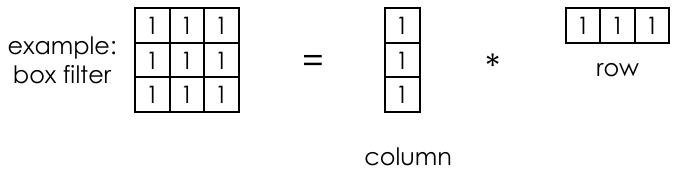
\includegraphics[width=0.8\textwidth]{img/separable_filter.png}
    \caption{Ejemplo de un filtro $2D$ separable que se descompone en dos filtros $1D$.}
    \label{fig:separable_filter}
\end{figure}

\noindent
La convolución $2D$ con un filtro separable es matemáticamente equivalente a realizar dos convoluciones $1D$ consecutivas (una con el filtro de columna y otra con el de fila). Esto tiene un impacto significativo en la eficiencia computacional. Si aplicamos un filtro de tamaño tamaño $K \times K$ (por ejemplo, un filtro de $3 \times 3$, donde $K=3$), para calcular un solo píxel de la imagen de salida, el ordenador tiene que:
\begin{enumerate}
    \item Poner el kernel sobre el píxel correspondiente.
    \item Multiplicar cada uno de los valores del kernel por el píxel que tiene debajo.
    \begin{itemize}
        \item En un kernel de $3 \times 3$, hay 9 valores. Por tanto, hacemos 9 multiplicaciones ($3^2 = 9$).
    \end{itemize}
    \item Sumar esos 9 resultados para obtener el valor final.
\end{enumerate}
Si generalizamos a un kernel de tamaño $K \times K$, para cada píxel de la imagen realizamos $K^2$ multiplicaciones. Si tu imagen tiene $N \times N$ píxeles, el coste total es $N^2 \cdot K^2$. \\ \\

\noindent
Sin embargo, si el filtro es separable, hemos dicho que $H = h_{col} \cdot h_{row}^T$. Esto significa que podemos descomponer la operación en dos pasos:

\begin{enumerate}
    \item Filtrado Horizontal: Pasamos un kernel de $1 \times K$ (una fila). Para cada píxel, solo hacemos $K$ multiplicaciones. Resultado: Una imagen intermedia.
    \item Filtrado Vertical: Sobre la imagen intermedia, pasamos un kernel de $K \times 1$ (una columna). Para cada píxel, hacemos otras $K$ multiplicaciones. Resultado: La imagen final.
\end{enumerate}
En total, para cada píxel tenemos que 
\begin{equation*}
    K \text{ (del horizontal)} + K \text{ (del vertical)} = 2K \text{ multiplicaciones}
\end{equation*}
esto representa una mejora significativa en términos de rendimiento, especialmente para filtros grandes. En lugar de $K^2$ multiplicaciones por píxel, solo necesitamos $2K$, lo que es una reducción drástica en la cantidad de cálculos necesarios para procesar la imagen. \\

\subsection{Padding}
\noindent
Cuando aplicas un filtro (convolución) usando un kernel (por ejemplo, una ventana de $3\times3$ o $5\times5$), necesitas posicionar el centro del kernel sobre cada píxel de la imagen. El problema surge en los píxeles de los bordes y esquinas: el kernel ``sobresale'' de la imagen, encontrándose con una zona vacía donde no existen píxeles. El \tbf{padding} es la estrategia matemática que usamos para rellenar ese vacío artificialmente. \\

\noindent
Las 4 estrategias usadas son las siguientes:
\begin{itemize}
    \item \tbf{Zero-padding (Recorte o Relleno con Ceros)}: asume que todos los píxeles fuera de los límites de la imagen original tienen un valor de cero (color negro).
    \item \tbf{Wrap / Periodic (Envoltura o Periódico)}: trata la imagen como si fuera una estructura cilíndrica o toroidal repetitiva. sta estrategia consiste en pegar los bordes opuestos de la imagen para darle continuidad:
    \begin{itemize}
        \item Pegas el borde derecho con el borde izquierdo, formando un cilindro.
        \item Pegas el borde superior con el borde inferior.
    \end{itemize}
    al hacer esto si el filtro (kernel) se sale por el lado derecho de la imagen, los píxeles que utiliza para rellenar ese vacío son los que están en el extremo izquierdo de esa misma fila.
    \item \tbf{Clamp / Replicate (Fijar o Replicar)}: extiende la imagen repitiendo el valor del último píxel disponible del borde de manera infinita hacia afuera.
    \item \tbf{Reflect / Mirror (Reflexión o Espejo)}: refleja los píxeles del interior de la imagen hacia el exterior, como si el borde fuera un espejo plano.
\end{itemize}


\subsection{Key filters}

\subsubsection{Box filter (Mean filter)}
\noindent
El \tbf{filtro de caja} (box filter) o \tbf{filtro de media} (mean filter) es un ejemplo clásico de filtro lineal que se utiliza para suavizar imágenes. Su kernel es una matriz donde todos los valores son iguales y suman 1. Por ejemplo, para un filtro de $3 \times 3$, el kernel sería
$$H = \frac{1}{9} \begin{bmatrix}
1 & 1 & 1 \\
1 & 1 & 1 \\
1 & 1 & 1
\end{bmatrix}$$
Este filtro es separable, ya que se puede descomponer en dos filtros $1D$:
\begin{equation*}
    h_{col} = \frac{1}{3} \begin{bmatrix}
1 \\
1 \\
1
\end{bmatrix}, \quad h_{row}^T = \frac{1}{3} \begin{bmatrix}
1 & 1 & 1
\end{bmatrix}
\end{equation*}
Al aplicar este filtro a una imagen, cada píxel de la imagen de salida se calcula como el promedio de los píxeles vecinos en la imagen original, lo que resulta en una imagen suavizada. Sin embargo, el filtro de caja puede introducir artefactos no deseados, como bordes borrosos y pérdida de detalles finos, especialmente cuando se utilizan kernels grandes. Además, debido a que todos los píxeles vecinos tienen el mismo peso, el filtro de caja no es tan efectivo para reducir el ruido sin afectar significativamente los bordes, lo que puede ser problemático en aplicaciones donde la preservación de los detalles es importante.

\subsubsection{Gaussian filter}
\noindent
El \tbf{filtro Gaussiano} se basa en la función de distribución normal (Gaussiana). En 2D, la función del kernel $G(x, y)$ viene dada por

$$G(x, y) = \frac{1}{2\pi\sigma^2} e^{-\dfrac{x^2 + y^2}{2\sigma^2}}$$
donde
\begin{itemize}
    \item $(x, y)$: son las coordenadas relativas al centro del kernel.
    \item $\sigma$ (Sigma): es la desviación estándar. Es el parámetro más importante, ya que define el ancho de la campana y, por tanto, el ``grado'' de desenfoque.
    \item $e$: es la base del logaritmo natural.
\end{itemize}
A diferencia del filtro de caja (\tbf{mean/box filter}) donde todos los valores son iguales (ej. todos 1/9), en el filtro Gaussiano el valor máximo está en el centro del kernel y va disminuyendo suavemente a medida que nos alejamos del centro, siguiendo la forma de una campana de Gauss. Esto significa que los píxeles más cercanos al centro del kernel tienen un mayor peso en la suma ponderada, mientras que los píxeles más alejados contribuyen menos al resultado final. \\


\subsubsection{Sharpen filter}
\noindent
El \tbf{filtro de nitidez} (sharpen filter) es un tipo de filtro que se utiliza para realzar los bordes y detalles finos en una imagen. A menudo, se construye a partir de la combinación de un filtro de suavizado (como el filtro de caja o el filtro Gaussiano) con la imagen original. La idea es restar la versión suavizada de la imagen original para obtener una máscara de alta frecuencia que resalte los detalles, y luego sumar esta máscara a la imagen original para obtener una imagen más nítida. \\

\noindent
El proceso matemático es el siguiente
\begin{equation*}
    \text{Detalles} = \text{Original} - \text{Suavizada}
\end{equation*}
Si restamos a la imagen original su versión borrosa, nos quedamos solo con los bordes y cambios bruscos. Si luego le sumamos eso a la original, los bordes se acentúan, es decir, tenemos que
\begin{equation*}
    \text{Sharpened} = \text{Original} + \alpha \cdot \text{Detalles}
\end{equation*}
donde $\alpha$ es un factor de control que determina cuánto queremos realzar los bordes, de manera que 
\begin{itemize}
    \item Si $\alpha = 0$, no hay realce y la imagen de salida es igual a la original.
    \item Si $\alpha > 0$, los bordes se acentúan.
    \item Si $\alpha < 0$, se produce un efecto de suavizado adicional.
\end{itemize}
De forma más matemática queda como
$$f_{sharp}(x,y) = f(x,y) + \alpha [f(x,y) - f_{smooth}(x,y)]$$
donde 
\begin{itemize}
    \item $f(x,y)$: es la imagen original.
    \item $f_{smooth}(x,y)$: es la versión suavizada de la imagen (obtenida mediante un filtro de caja o Gaussiano).
    \item $\alpha$: es un factor que controla cuánto queremos realzar los bordes.
\end{itemize}
Si operamos la fórmula, tenemos
$$f_{sharp} = (1+\alpha)f - \alpha f_{smooth}$$

\section{Non-linear filtering}
\noindent 
Entender concepto solo, no es necesario memorizar fórmulas (no es pregunta de examen). \\

\noindent
A diferencia de los lineales (como el promedio o el Gaussiano), donde el resultado es una suma ponderada de los vecinos, en los filtros no lineales la operación no puede expresarse como una matriz de pesos fija (kernel). El valor de salida depende de una regla lógica o estadística aplicada a la vecindad.


\subsubsection{Bilateral filter}

\noindent
El filtro \tbf{bilateral} es un filtro no lineal que se utiliza para suavizar imágenes mientras preserva los bordes, por lo que se presenta como una evolución avanzada del filtro Gaussiano, diseñada para resolver su principal problema: el desenfoque de los bordes. Mientras que el filtro Gaussiano es un filtro "ciego" que suaviza todo por igual, el filtro bilateral es un filtro \underline{preservador de bordes} (edge-preserving). \\ \\
\noindent
Si aplicamos un filtro Gaussiano estándar en una zona donde hay un borde (un cambio brusco de intensidad), el filtro mezclará los píxeles de ambos lados del borde, emborronándolo. El filtro bilateral, en cambio, solo promedia aquellos píxeles que son cercanos en el espacio $Y$ similares en intensidad. \\ \\
\noindent
A diferencia del filtro Gaussiano que solo tiene un componente, el filtro bilateral combina dos funciones Gaussianas. El valor del píxel de salida $g(x, y)$ se calcula como:

$$g(x, y) = \frac{1}{W_p} \sum_{u, v} f(x+u, y+v) \cdot G_{\sigma_s}(u,v) \cdot G_{\sigma_r}(| f(x,y) - f(x+u,y+v) |)$$
donde 
\begin{itemize}
    \item $G_{\sigma_s}$ (Domain Kernel): es la Gaussiana espacial que ya conoces. Da más peso a los píxeles que están cerca físicamente. Depende de la distancia en coordenadas.
    \item $G_{\sigma_r}$ (Range Kernel): es la ``magia'' del filtro. Da más peso a los píxeles que tienen un valor de intensidad (color) similar al píxel central. Depende de la diferencia de brillo.
    \item $W_p$: es un factor de normaliçzación para asegurar que la suma de los pesos sea 1.
\end{itemize}


\subsubsection{Filtro de la mediana (Median Filter)}
\noindent
Es el filtro no lineal más famoso y utilizado. En lugar de promediar los píxeles de la ventana, los ordena de menor a mayor y selecciona el valor que queda justo en la posición central (la mediana). Es extremadamente eficaz para eliminar el ruido de ``sal y pimienta'' (puntos blancos y negros aleatorios). Se puede ver un ejemplo de este ruido en la Figura \ref{fig:median_filter}.

\begin{figure}[h]
    \centering
    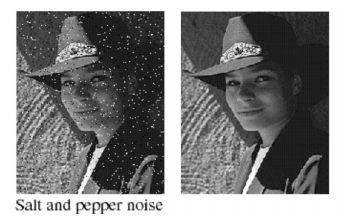
\includegraphics[width=0.8\textwidth]{img/median_filter.png}
    \caption{Ejemplo de filtro de la mediana.}
    \label{fig:median_filter}
\end{figure}

\subsubsection{Threshold filter}
\noindent
El threshold filter es una de las operaciones de punto más sencillas pero más potentes en el procesado de imágenes. Se utiliza principalmente para la segmentación, es decir, para separar los objetos del fondo. \\ \\
\noindent
Consiste en comparar cada píxel de la imagen con un valor constante llamado umbral ($T$). Dependiendo de esa comparación, el píxel se transforma en uno de dos valores posibles (normalmente blanco o negro). Viene dado de esta manera
$$g(x, y) =\begin{cases}255 & \text{si } f(x, y) > T \\ 0 & \text{si } f(x, y) \leq T\end{cases}$$
donde 
\begin{itemize}
    \item $f(x, y)$: intensidad del píxel original.
    \item $T$: el umbral (un valor entre 0 y 255).
    \item $g(x, y)$: imagen binaria resultante.
\end{itemize}

\section{Sampling y Aliasing}
\noindent 
Entender concepto solo, no es necesario memorizar fórmulas (no es pregunta de examen). \\

\noindent
El \tbf{aliasing} es un defecto visual que ocurre cuando la \tbf{tasa de muestreo} (sampling rate) que utilizamos no es lo suficientemente alta para capturar toda la cantidad de detalle fino presente en la imagen. \\

\begin{definicion}
    La \tbf{tasa de muestreo} es la densidad de píxeles (píxeles por milímetro o la resolución total de la cuadrícula de tu sensor de cámara). Si una imagen tiene $N \times N$ pixeles, entonces la tasa de muestreo es $N$ por cada eje.
\end{definicion}
\noindent
Visualmente, esto se traduce en artefactos engañosos, como patrones extraños, anillos o bordes aserrados que no existían en la imagen original. Al perderse información clave, obtenemos una imagen que representa una señal incorrecta, lo que se conoce como un ``alias''.  \\\\
\noindent
Para evitar el aliasing y realizar el muestreo correctamente, la teoría del procesamiento de señales se apoya en el \tbf{Teorema de muestreo de Nyquist-Shannon}, que indica que para no perder información y no generar aliasing al reducir una imagen, la tasa de muestreo debe ser al menos el doble de la frecuencia máxima presente en la imagen, e decir
\begin{equation*}
    f_s \geq 2 \cdot f_{max}
\end{equation*}
A esta tasa de muestreo mínima requerida se le llama la \tbf{Tasa de Nyquist}.

\subsubsection{Subsampling y Upsampling}

\noindent
El proceso para conseguir el \tbf{subsampling} de forma correcta es el siguiente, si queremos reducir el tamaño de una imagen (por ejemplo, a la mitad), estamos reduciendo la cantidad de píxeles disponibles para representar la información. Esto significa que la frecuencia máxima que podemos representar también se reduce. Si no hacemos nada para eliminar las frecuencias altas antes de reducir el tamaño, esas frecuencias se convertirán en alias (artefactos) en la imagen reducida, por lo que hacemos es lo siguiente
\begin{enumerate}
    \item \tbf{Analizamos la nueva tasa}: Si vamos a reducir la imagen a la mitad, nuestra nueva frecuencia máxima permitida (Límite de Nyquist) es ahora mucho más baja.
    \item \tbf{Aplicamos el filtro}: Pasamos un filtro Gaussiano que actúa como un filtro de paso bajo. Su función es eliminar (emborronar) todos los detalles cuya frecuencia sea mayor que el nuevo límite de Nyquist.
    \item \tbf{Muestreamos}: Ahora que hemos ``limpiado'' las frecuencias prohibidas, podemos quitar píxeles de forma segura (por ejemplo, nos quedamos con uno de cada dos píxeles).
\end{enumerate}
Esto se formaliza al construir la \tbf{Pirámide Gaussiana}, donde cada nivel $l$ de la pirámide se obtiene del nivel anterior $l-1$ mediante: convolución con un kernel Gaussiano (normalmente con un $\sigma$ específico para esa escala), y después eliminación de cada segunda fila y columna.

$$G_l = \text{subsample}(G_{l-1} * \text{Gaussian})$$
Si omitiéramos el paso del filtro, la imagen resultante en el nivel superior estaría llena de ruido y errores de aliasing. Al filtrar, nos aseguramos de que la información que queda es una representación fiel, aunque menos detallada, de la original. \\ \\

\noindent
Ahora nos centraremos en ver cómo podemos hacer el proceso contrario, es decir, el \tbf{upsampling} o aumento de tamaño. En este caso, el proceso es el siguiente
\begin{enumerate}
    \item \tbf{Muestreamos}: si tenemos una imagen de $N \times N$, creamos una nueva matriz de $2N \times 2N$, donde colocamos los píxeles originales en las posiciones pares y rellenamos los nuevos huecos con ceros.
    \item \tbf{Aplicamos el filtro}: Pasamos un filtro Gaussiano para suavizar la imagen resultante. Esto es necesario porque al insertar nuevos píxeles sin información real, obtenemos una imagen con bordes muy duros y artefactos. El filtro ayuda a interpolar esos nuevos píxeles de manera más natural.
\end{enumerate}
Matemáticamente, el proceso de upsampling se puede expresar como:
$$G_{l-1} = \text{upsample}(G_l) * \text{Gaussian}$$
donde $G_l$ es la imagen en el nivel actual de la pirámide, y $G_{l-1}$ es la imagen resultante después de el upsampling y el filtrado. El resultado final es una imagen más grande y suave.

\section{Image derivatives}
\noindent 
Entender concepto solo, no es necesario memorizar fórmulas (no es pregunta de examen). \\

\noindent
Un \tbf{borde} es, por definición, una zona donde la intensidad de los píxeles cambia de forma brusca (por ejemplo, pasamos de un fondo negro a un objeto blanco). Matemáticamente, un cambio brusco genera una derivada con un valor alto. Al derivar la imagen, convertimos las zonas planas en negro (valor 0, ya que no hay cambio) y resaltamos los bordes en blanco. \\ 

\noindent
Como tenemos dos dimensiones ($x, y$), calculamos las variaciones en ambas direcciones:
\begin{itemize}
    \item \tbf{Derivada en X ($\frac{\partial f}{\partial x}$)}: detecta cambios de intensidad horizontales (bordes verticales), se mira el píxel que está a la derecha del píxel actual y el que está a la izquierda, y resta sus valores de brillo.
    \item \tbf{Derivada en Y ($\frac{\partial f}{\partial y}$)}: detecta cambios de intensidad verticales (bordes horizontales), se mira el píxel que está justo abajo del píxel actual y el que está justo arriba, y resta sus valores de brillo.
\end{itemize}
Matemáticamente, en el mundo discreto de los píxeles, usamos la aproximación de diferencia finita
$$\frac{\partial f}{\partial x} \approx f(x+1, y) - f(x, y)$$
Podemos ver un ejemplo en la Figura \ref{fig:image_derivatives}.
\begin{figure}[h]
    \centering
    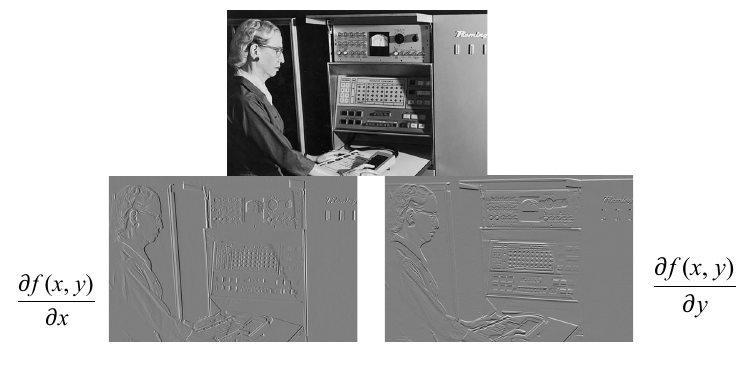
\includegraphics[width=0.8\textwidth]{img/image_derivates.png}
    \caption{Ejemplo de derivadas de la imagen.}
    \label{fig:image_derivatives}
\end{figure}

\noindent
El \tbf{gradiente} es un vector que agrupa ambas derivadas parciales
$$\nabla f = \left[ \frac{\partial f}{\partial x}, \frac{\partial f}{\partial y} \right]$$
De este vector extraemos dos piezas de información críticas para cualquier algoritmo de visión:
\begin{itemize}
    \item \tbf{Magnitud del Gradiente}: Indica la ``fuerza" del borde. Se calcula como 
    $$\|\nabla f\| = \sqrt{\left(\frac{\partial f}{\partial x}\right)^2 + \left(\frac{\partial f}{\partial y}\right)^2}$$
    \item \tbf{Orientación del Gradiente}: Indica la dirección del cambio de intensidad más rápido. Se calcula como 
    $$\theta = \tan^{-1}\left(\frac{\partial f / \partial y}{\partial f / \partial x}\right)$$
\end{itemize}
Podemos ver un ejemplo en la Figura \ref{fig:gradient_magnitude_orientation}, donde se muestra la magnitud y orientación del gradiente para una imagen dada. \\ \\

\begin{figure}
    \centering
    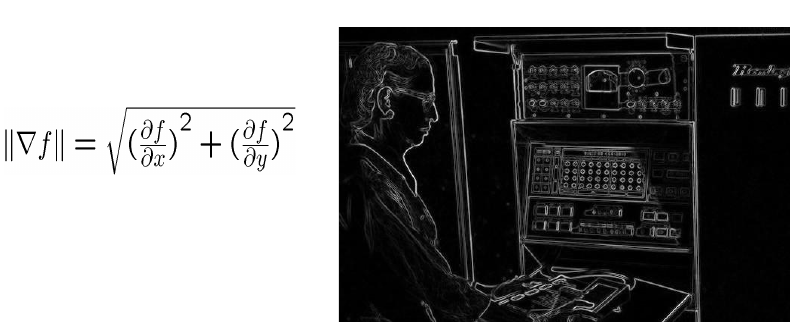
\includegraphics[width=0.8\textwidth]{img/gradient_magnitude_orientation.png}
    \caption{Ejemplo de magnitud y orientación del gradiente.}
    \label{fig:gradient_magnitude_orientation}
\end{figure}

\noindent
Hay que tener en cuenta que las derivadas son muy sensibles al ruido, por lo que es común aplicar un filtro de suavizado (como el Gaussiano) antes de calcular las derivadas para obtener resultados más estables y precisos. En este proceso solemos usar el \tbf{Teorema de la Convolución}, que nos dice que la convolución de una imagen con la derivada de un filtro es equivalente a calcular la derivada de la imagen suavizada con ese filtro. Esto se expresa matemáticamente como:
$$\frac{\partial}{\partial x}(f * G) = f * \frac{\partial G}{\partial x}$$
Esto significa que podemos pre-calcular la derivada del filtro Gaussiano (que es un filtro de Sobel, veremos más adelante qué es eso) y luego convolucionarlo con la imagen original, en lugar de tener que suavizar la imagen primero y luego calcular la derivada. Esto es mucho más eficiente computacionalmente y nos da el mismo resultado.

\section{Edge detection}
\noindent
Otra forma de encontrar bordes es utilizando filtros de segunda derivada, como el \tbf{filtro Laplaciano}. En la segunda derivada, un borde ya no es un ``pico'', sino el punto exacto donde la función cruza el valor de cero. A esto se le llama cruce por cero (\tbf{zero-crossing}), y tiene la ventaja de que es computacionalmente más fácil de localizar que buscar un valor máximo. Matemáticamente, el filtro Laplaciano se define como la suma de las segundas derivadas parciales:
$$\nabla^2 f = \frac{\partial^2 f}{\partial x^2} + \frac{\partial^2 f}{\partial y^2}\implies LoG=\nabla^2 (G_\sigma \ast f)=\nabla^2(G_\sigma)\ast f$$
que se va a aproximar de esta manera
$$\frac{\partial^2 f}{\partial x^2} \approx f(x+1) - 2f(x) + f(x-1)$$
donde $LoG$ es el filtro de Laplaciano de Gaussiano, que se obtiene aplicando el filtro de Laplaciano a la imagen suavizada con un filtro Gaussiano. El proceso de detección de bordes con el filtro Laplaciano implica buscar los puntos donde el resultado del filtro cambia de signo (de positivo a negativo o viceversa), lo que indica la presencia de un borde.

\subsection{Derivatives filters}
\subsubsection{Sobel filter}
\noindent
El \tbf{filtro de Sobel} se utiliza para aproximar la primera derivada de la imagen. Su objetivo es calcular el gradiente de la intensidad en cada píxel, lo que nos indica la fuerza de un borde y su dirección. La clave del Sobel es que combina dos operaciones en una sola matriz:

\begin{itemize}
    \item \tbf{Diferenciación}: cacula la diferencia de intensidad (derivada).
    \item \tbf{Suavizado}: aplica un pequeño desenfoque (promedio pesado) en la dirección perpendicular a la derivada para reducir el ruido.
\end{itemize}
Para obtener el gradiente completo, aplicamos dos filtros independientes, uno para la dirección horizontal y otro para la vertical. Típicamente son matrices de $3 \times 3$:
\begin{itemize}
    \item \textbf{Gradiente Horizontal ($G_x$)}: Detecta bordes verticales. Su kernel es:
$$S_x = \dfrac{1}{8}\begin{bmatrix} -1 & 0 & 1 \\ -2 & 0 & 2 \\ -1 & 0 & 1 \end{bmatrix} \implies G_x=S_x\ast f $$
    \item \textbf{Gradiente Vertical ($G_y$)}: Detecta bordes horizontales. Su kernel es:
$$S_y = \dfrac{1}{8}\begin{bmatrix} 1 & 2 & 1 \\ 0 & 0 & 0 \\ -1 & -2 & -1 \end{bmatrix} \implies G_y=S_y\ast f$$
\end{itemize}
aunque la versión estándar no tiene la normalización de $1/8$, se suele incluir para mantener los valores dentro del rango de intensidad. Al aplicar estos filtros a la imagen, obtenemos dos imágenes de gradiente ($G_x$ y $G_y$) que representan la fuerza de los bordes en las direcciones horizontal y vertical, respectivamente. Luego, podemos combinar estas dos imágenes para obtener la magnitud del gradiente total, que nos da una medida de la fuerza del borde en cada píxel. De hecho, el filtro de Sobel es \underline{separable}, veámoslo
$$\begin{bmatrix} -1 & 0 & 1 \\ -2 & 0 & 2 \\ -1 & 0 & 1 \end{bmatrix} = \begin{bmatrix} 1 \\ 2 \\ 1 \end{bmatrix} * \begin{bmatrix} -1 & 0 & 1 \end{bmatrix}$$
donde tenemos 
\begin{itemize}
    \item Filtro Vertical: 
    $$\begin{bmatrix} 1 & 2 & 1 \end{bmatrix}^T$$
    es un componente de suavizado (smoothing). Al tener valores positivos, promedia los píxeles de las filas adyacentes, lo que ayuda a reducir el ruido antes de calcular la diferencia.
    \item Filtro Horizontal: 
    $$\begin{bmatrix} -1 & 0 & 1 \end{bmatrix}$$
    es el componente de diferenciación (derivada). Es el que realmente calcula la diferencia de intensidad entre el lado izquierdo y el derecho para detectar el borde.
\end{itemize}
Lo que podemos ver aqui es que el operador de Sobel no es más que una derivada suavizada, pues si solo usáramos $[-1, 0, 1]$, el ruido afectaría mucho al resultado, pero al multiplicarlo por $[1, 2, 1]^T$, estamos diciendo: ``calcula la derivada, pero dale más importancia a la fila central y promedia un poco con las filas de arriba y abajo para que el resultado sea más estable''. Podemos ver un ejemplo del resultado de ambos gradientes en la Figura \ref{fig:gradientes_sobel}.\\

\begin{figure}
    \centering
    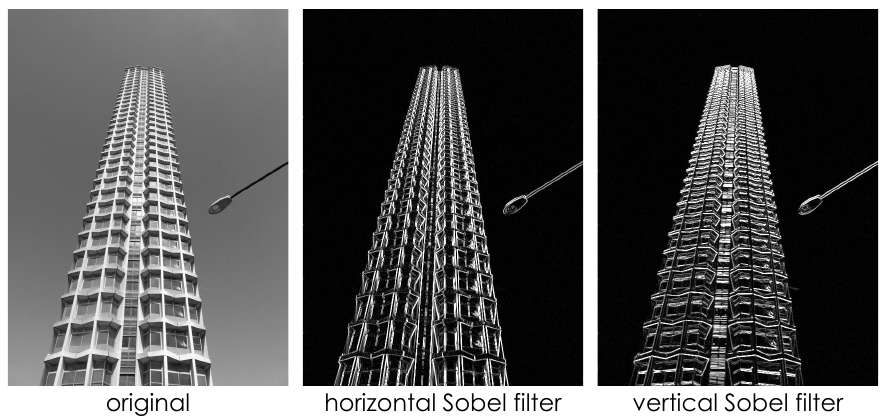
\includegraphics[width=0.8\textwidth]{img/gradientes_sobel.png}
    \caption{Ejemplo de los gradientes $G_x$ y $G_y$ obtenidos al aplicar el filtro de Sobel a una imagen.}
    \label{fig:gradientes_sobel}
\end{figure}

\noindent
El resultado final de aplicar Sobel, es unir ambos gradientes, $G_x$ y $G_y$, para obtener la magnitud del gradiente total, que nos da una medida de la fuerza del borde en cada píxel. Esto se calcula como:
$$M(x, y) = \sqrt{G_x(x, y)^2 + G_y(x, y)^2}\quad \equiv \quad M = \sqrt{G_x^2 + G_y^2}$$
y la orientación del borde se calcula como
$$\theta(x,y) = \tan^{-1}\left(\frac{G_y(x, y)}{G_x(x, y)}\right) \quad \equiv \quad \theta = \tan^{-1}\left(\frac{G_y}{G_x}\right)$$
\begin{observacion}
    La orientación del borde no es estrictamente necesaria si solo aplicamos el filtro de Sobel, pero veremos más adelante su uso en otros casos. \\
\end{observacion}
\noindent
El filtro de Sobel es ampliamente utilizado en aplicaciones de visión por computadora para la detección de bordes, ya que proporciona una buena aproximación de la derivada de la imagen mientras reduce el impacto del ruido, lo que lo hace ideal para detectar bordes en imágenes reales que a menudo contienen ruido. \\

\noindent
El \tbf{resultado final} de aplicar el filtro de Sobel a una imagen es una nueva imagen donde los bordes se resaltan como líneas brillantes (blancas) sobre un fondo oscuro. La intensidad de estas líneas blancas corresponde a la fuerza del borde detectado, es decir, a la magnitud del gradiente en esa región.\\

\observacion{
    Es normal que al aplicar Sobel, el resultado nos de líneas blancas gruesas que marquen los bordes, puesto que el filtro de Sobel no solo detecta el borde, sino que también lo suaviza, lo que hace que el borde resultante tenga un grosor de varios píxeles. Para obtener bordes más delgados, se pueden aplicar técnicas adicionales como la supresión de no-máximos (non-maximum suppression) o utilizar filtros de derivada más precisos como el filtro de Canny, que veremos a continuación.\\
}

\noindent
Podemos ver un ejemplo en la Figura \ref{fig:sobel_canny} de la diferencia de aplicar el filtro de Sobel y Canny, para ver como en el primer caso las líneas de los bordes son más gruesas.

\begin{figure}
    \centering
    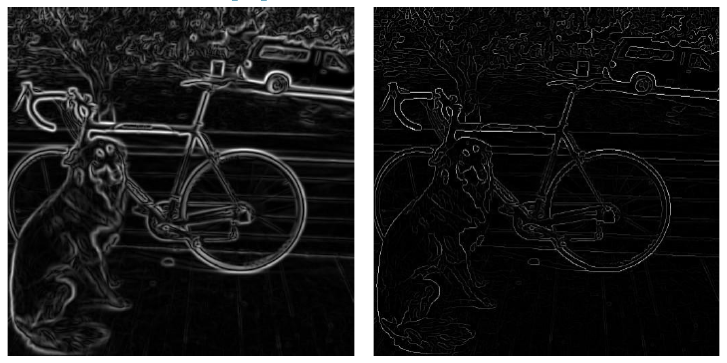
\includegraphics[width=0.8\textwidth]{img/sobel_canny.png}
    \caption{Comparación bordes entre filtro de Sobel (izquierda) y algoritmo de Canny (derecha).}
    \label{fig:sobel_canny}
\end{figure}

\subsection{Canny Edge Detector}
\noindent
No es simplemente un filtro, sino nuestro primer pipeline completo de Computer Vision. Fue diseñado por John Canny en 1986 con el objetivo de ser el ``detector óptimo'' basándose en tres criterios: baja tasa de error, buena localización y respuesta única. El algoritmo se divide en cuatro pasos fundamentales, veámoslo
\begin{enumerate}
    \item \tbf{Suavizado (Smoothing)}: El primer paso es aplicar un filtro Gaussiano para eliminar el ruido de alta frecuencia que podría generar bordes falsos, es decir, aplicar
    \begin{equation*}
            fs = G_\sigma \ast f \quad \text{(eliminar ruido)}
    \end{equation*}
    \item \tbf{Cálculo del Gradiente}: Se calcula la magnitud y la orientación del gradiente utilizando operadores de derivada (como Sobel). La magnitud ($M$) indica la fuerza del cambio de intensidad, mientras que la orientación ($\theta$) indica la dirección perpendicular al borde, véamolos
    \begin{equation*}
        M = \|\nabla fs\| \quad \text{ y } \quad \theta = \tan^{-1}\left(\frac{\partial fs / \partial y}{\partial fs / \partial x}\right)
    \end{equation*}
    \item \tbf{Supresión de No-Máximos (Non-maximum Suppression)}: este paso es el que hace que Canny sea \underline{especial}. El objetivo es ``adelgazar'' los bordes para que tengan solo 1 píxel de grosor. \\
    \noindent
    Cómo funciona: el algoritmo recorre cada píxel y comprueba si su magnitud es un máximo local en la dirección de su gradiente. Lo que hacemos es aislar un vector de 3 píxeles, de manera que solo comparamos el píxel central con sus dos vecinos en la dirección del gradiente, de la siguiente manera
    \begin{itemize}
        \item Si el píxel central tiene una magnitud mayor que ambos vecinos, se mantiene su valor.
        \item Si no es un máximo local, se pone a cero.
    \end{itemize}
    Esto convierte las ``rampas'' de intensidad en líneas finas y precisas.
    \item \tbf{Umbralización por Histéresis (Hysteresis Thresholding)}: en lugar de usar un solo umbral (que podría romper un borde si su intensidad varía ligeramente), Canny utiliza dos umbrales: uno Alto ($T_h$) y uno Bajo ($T_l$), de la siguiente manera
    \begin{itemize}
        \item \underline{Píxeles Fuertes}: Si la magnitud $> T_h$, se acepta como borde definitivo.
        \item \underline{Píxeles Débiles}: Si $T_l < \text{magnitud} < T_h$, solo se acepta como borde si está conectado a un píxel fuerte.
        \item \underline{Ruido}: Si la magnitud $< T_l$, se descarta.
    \end{itemize}
    El objetivo de este proceso, es asegurar que las líneas que marquen los bordes tengan una intensidad mínima, y que en los casos en los que una píxel de esa linea que define un borde tenga menos intensidad, antes de eliminarlo completamente, comprobamos si está conectado a un borde fuerte, lo que nos permite mantener bordes completos incluso si su intensidad varía a lo largo de su longitud. Podemos ver un ejemplo de esta ultima fase en la Figura \ref{fig:hysteresis_thresholding}.
    \begin{observacion}
        Para ver si está conectado a un pixel fuerte, como bien se hace en el ejemplo de la figura, cogeremos los píxeles de su entorno (los 8 de su alrededor).
    \end{observacion}
\end{enumerate}

\begin{figure}
    \centering
    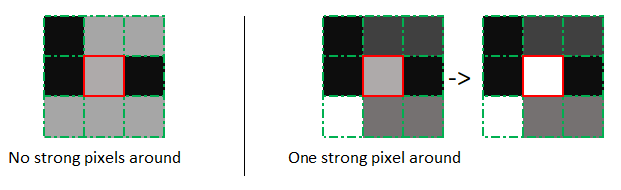
\includegraphics[width=0.8\textwidth]{img/hysteresis_thresholding.png}
    \caption{Ejemplo de umbralización por histéresis en el algoritmo de Canny.}
    \label{fig:hysteresis_thresholding}
\end{figure}
Podemos ver un resumen de este tema en la Figura \ref{fig:summary2}.

\begin{figure}[h]
    \centering
    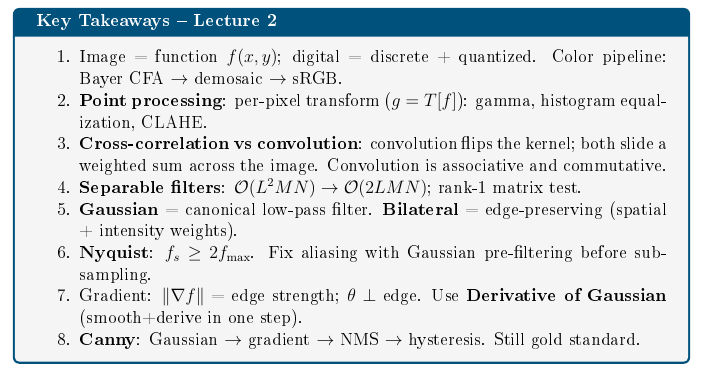
\includegraphics[width=0.8\textwidth]{img/summary2.png}
    \caption{Resumen de Tema 2.}
    \label{fig:summary2}
\end{figure}